\documentclass[10pt]{article}



\usepackage{amsmath,amscd}
\usepackage{amssymb,array}
\usepackage{amsfonts,latexsym}
\usepackage{graphicx,subfig,wrapfig}
\usepackage{times}
\usepackage{psfrag,epsfig}
\usepackage{verbatim}
\usepackage{tabularx}
\usepackage[pagebackref=true,breaklinks=true,letterpaper=true,colorlinks,bookmarks=false]{hyperref}
\usepackage{cite}
\usepackage{algorithm}
\usepackage{multirow}
\usepackage{caption}
\usepackage{algorithmic}
\usepackage[amsmath,thmmarks]{ntheorem}
\usepackage{listings}
\usepackage{color}


\newtheorem{thm}{Theorem}
\newtheorem{mydef}{Definition}

\DeclareMathOperator*{\rank}{rank}
\DeclareMathOperator*{\trace}{trace}
\DeclareMathOperator*{\acos}{acos}
\DeclareMathOperator*{\argmax}{argmax}


\renewcommand{\algorithmicrequire}{ \textbf{Input:}}     
\renewcommand{\algorithmicensure}{ \textbf{Output:}}
\renewcommand{\mathbf}{\boldsymbol}
\newcommand{\mb}{\mathbf}
\newcommand{\matlab}[1]{\texttt{#1}}
\newcommand{\setname}[1]{\textsl{#1}}
\newcommand{\Ce}{\mathbb{C}}
\newcommand{\Ee}{\mathbb{E}}
\newcommand{\Ne}{\mathbb{N}}
\newcommand{\Se}{\mathbb{S}}
\newcommand{\norm}[2]{\left\| #1 \right\|_{#2}}

\newenvironment{mfunction}[1]{
	\noindent
	\tabularx{\linewidth}{>{\ttfamily}rX}
	\hline
	\multicolumn{2}{l}{\textbf{Function \matlab{#1}}}\\
	\hline
}{\\\endtabularx}

\newcommand{\parameters}{\multicolumn{2}{l}{\textbf{Parameters}}\\}

\newcommand{\fdescription}[1]{\multicolumn{2}{p{0.96\linewidth}}{
		
		\textbf{Description}
		
		#1}\\\hline}

\newcommand{\retvalues}{\multicolumn{2}{l}{\textbf{Returned values}}\\}
\def\0{\boldsymbol{0}}
\def\b{\boldsymbol{b}}
\def\bmu{\boldsymbol{\mu}}
\def\e{\boldsymbol{e}}
\def\u{\boldsymbol{u}}
\def\x{\boldsymbol{x}}
\def\v{\boldsymbol{v}}
\def\w{\boldsymbol{w}}
\def\N{\boldsymbol{N}}
\def\X{\boldsymbol{X}}
\def\Y{\boldsymbol{Y}}
\def\A{\boldsymbol{A}}
\def\B{\boldsymbol{B}}
\def\y{\boldsymbol{y}}
\def\cX{\mathcal{X}}
\def\transpose{\top} % Vector and Matrix Transpose

%\long\def\answer#1{{\bf ANSWER:} #1}
\long\def\answer#1{}
\newcommand{\myhat}{\widehat}
\long\def\comment#1{}
\newcommand{\eg}{{e.g.,~}}
\newcommand{\ea}{{et al.~}}
\newcommand{\ie}{{i.e.,~}}

\newcommand{\db}{{\boldsymbol{d}}}
\renewcommand{\Re}{{\mathbb{R}}}
\newcommand{\Pe}{{\mathbb{P}}}

\hyphenation{MATLAB}

\usepackage[margin=1in]{geometry}

\begin{document}
	
\title{Machine Learning, Spring 2018\\Homework 5}
\date{Due on 23:59 May 16, 2018\\Compress all your materials in {\color{red}one} file, and send to $cs282\_01@163.com$ \\with subject {\color{red}``Chinese name+student number+HW5'' (In this format please!)}}
\maketitle

%%%%%--------------------

\section*{Understanding VC dimension ($20$ points)} 

In this part, you need to complete some mathematical proofs about VC dimension. Suppose the hypothesis set
\begin{equation*}
\mathcal{H} = \{f(x, \alpha) = \mathrm{sign} \ ( \mathrm{sin}(\alpha x))|, \alpha \in \Re \}
\end{equation*}
where $x$ and $f$ are feature and label, respectively.
\begin{itemize}
	\item Show that $\mathcal{H}$ cannot shatter the points $x_1 = 1, x_2 = 2, x_3 = 3, x_4 = 4$. ($8$ points) \\
	
	
	(Key: Mathematically, you need to show that there exists $y_1, y_2, y_3, y_4$, for any $\alpha \in \Re$, $f(x_i) \neq y_i, i = 1,2,3,4$, for example, $+1, +1, -1, +1$)
	
	\item Show that the VC dimension of $\mathcal{H}$ is $\infty$. (Note the difference between it and the first question) ($12$ points) \\
	
	(Key: Mathematically, you have to prove that for any label sets ${y_1 , \cdots , y_m}, m \in \Ne $, there exists $\alpha \in \Re$ and $x_i, i = 1,2,\cdots,m$
	such that $f(x; \alpha)$ can generate this set of labels. Consider the points $x_i = 10^{-i}$...)
	
\end{itemize} 

\section*{Understanding Lasso ($30$ points)}
Consider the following generalized Lasso problem
\begin{equation} \label{glasso}
\begin{aligned}
\underset{\mb{x}} {\text{ min}} \  \frac{1}{2} \norm{\mb{A}\mb{x}-\mb{b}}{2}^2 + \lambda \norm{\mb{F}\mb{x}}{1}, 
\end{aligned}
\end{equation}
where $\mb{A}$ is the under-determined sensing matrix, $\mb{F}$ is the transformed matrix. In particular, it can be reduced to Lasso problem if $\mb{F} = \mb{I}$. The above problem is equivalent to the following formulation
\begin{equation} \label{glasso_adm}
\begin{aligned}
&\underset{\mb{x}, \mb{z}} {\text{ min}} \  \frac{1}{2} \norm{\mb{A}\mb{x}-\mb{b}}{2}^2 + \lambda \norm{\mb{z}}{1} \\
& \ \text{s.t.} \ \mb{F}\mb{x} = \mb{z},
\end{aligned}
\end{equation}
and one can employ augmented Lagrangian multiplier method to solve it. Specifically, the augmented Lagrangian is 
\begin{equation*}
\mathcal{L} = \frac{1}{2} \norm{\mb{A}\mb{x}-\mb{b}}{2}^2 + \lambda \norm{\mb{z}}{1} + <\mb{y}, \mb{F}\mb{x}- \mb{z}> + \frac{1}{2} \rho \norm{\mb{F}\mb{x} - \mb{z}}{2}^2,
\end{equation*}
which yields the ADMM algorithm, see Algorithm \ref{alg_glasso}. The soft-thresholding operator $\Se_{\frac{\lambda}{\rho}}$ is defined as 
\begin{equation}
\Se_{\frac{\lambda}{\rho}} (x_i) = \begin{cases}
x_i - \frac{\lambda}{\rho}, \ x_i \geq \frac{\lambda}{\rho} \\
0, \ |x_i| < \frac{\lambda}{\rho} \\
x_i + \frac{\lambda}{\rho}, \ x_i \leq -\frac{\lambda}{\rho}.
\end{cases}
\end{equation} 
\begin{algorithm}[h]
	\caption{ALM for generalized Lasso problem}
	\label{alg_glasso}
	\begin{algorithmic}[1] 
		\REQUIRE $\mb{A}, \mb{F}, \mb{b}, \lambda, \mu \ (\text{for augmented Lagrange multiplier})$
		\STATE Initialized $\rho, \mb{x}_0, \mb{z}_0,$ and $\mb{y}_0$, $k = 0$
		\WHILE {not converged}
		\STATE $\mb{x}^{(k+1)} = update \ \mb{x} ?$
		\STATE $\mb{z}^{(k+1)} = update \ \mb{z} ?$ (you may want to use $\Se_{\frac{\lambda}{\rho}}$ element-wise)
		\STATE $\mb{y}^{(k+1)} = \mb{y}^{(k)} + \rho (\mb{F} \mb{x}^{(k+1)} - \mb{z}^{(k+1)})$
		\STATE $\rho = \rho \mu$
		\STATE $k = k + 1$
		\ENDWHILE
		\ENSURE $\mb{x}^{*} = \mb{x}^{(k)}$
	\end{algorithmic}
\end{algorithm}

\begin{itemize}
	\item Derive the steps of update $\mb{x}$ and $\mb{z}$ in Algorithm \ref{alg_glasso}. ($10$ points)
	
	\item Complete the function \matlab{glasso.m}, and pass the test using \matlab{testglasso.m} ($15$ points)
	
	\item Run \matlab{demo.m} and report your MSE and PSNR. ($5$ points)
	
\end{itemize} 

\section*{Dual Formulation of the SVM ($25$ points)}
Compared with the SVM formulation in Lecture $15$ and $16$, its dual problem will be much eaiser, since the original problem has so many constraints.
\begin{itemize}
	\item Give the dual formulation of the SVM and what  the KKT condition is for primal SVM. We need you show the induction of the procedure. 
	\item There is a efficient for dual SVM problem, called Sequential Minimal Optimization. You can find many materials for this algorithm from website, it make use of the KKT conditios to solve the dual quadratic problem. 
	\begin{itemize}
		\item Give us an abstract of its principle and the pseudocode of the SMO algorithm for the dual SVM problem.
		\item \emph{a3a} is a data for the binary classification, show us your accuracy of the test data, like Fig~\ref{fig.3}. You need download the data \emph{a3a} from \url{https://www.csie.ntu.edu.tw/~cjlin/libsvmtools/datasets/}
		\begin{figure}[ht]
			\centering
			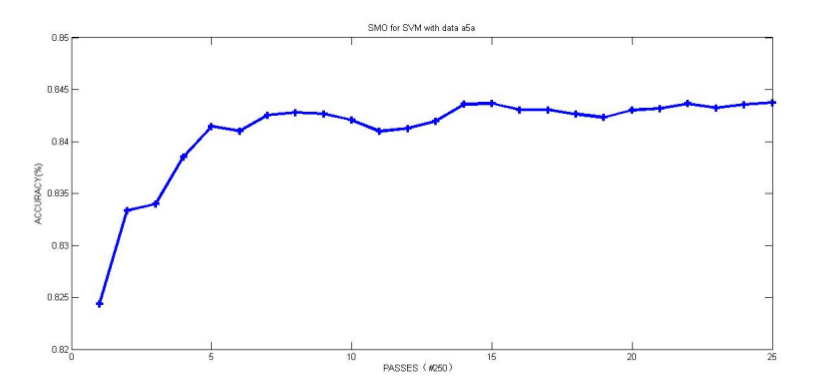
\includegraphics[width=0.8\linewidth]{fig1.png}
			\caption{Accuracy demo.}
			\label{fig.3}
		\end{figure}
	\end{itemize}
	
\end{itemize}

\section*{Kernel function ($25$ points)}
Suppose we are given the following positively (``$+1$'') labeled data points $\mathbb{R}^2$:
$$
\begin{Bmatrix}
\begin{pmatrix}
1\\ 
1
\end{pmatrix} ,&
\begin{pmatrix}
1\\ 
-1
\end{pmatrix}  ,&
\begin{pmatrix}
-1\\ 
1
\end{pmatrix} ,&
\begin{pmatrix}
-1\\ 
-1
\end{pmatrix}
\end{Bmatrix},
$$
and the following negatively labeled (``$-1$'') data points in $\mathbb{R}^2$ (see Figure~\ref{fig:svm}):
$$
\begin{Bmatrix}
\begin{pmatrix}
2\\ 
2
\end{pmatrix} ,&
\begin{pmatrix}
2\\ 
-2
\end{pmatrix}  ,&
\begin{pmatrix}
-2\\ 
2
\end{pmatrix} ,&
\begin{pmatrix}
-2\\ 
-2
\end{pmatrix}
\end{Bmatrix}.
$$
\begin{figure}[h!]
	\centering
	\includegraphics[width=3in]{svm.png}
	\caption{Blue diamonds are positive examples and red squares are negative examples.}
	\label{fig:svm}
\end{figure}	
\textbf{Question}: 
\begin{enumerate}
	\item Find a kernel function to map the data into a $\mathbb{R}^3$ feature space and make the new data linearly separable. (Show your kernel function please!) ($5$points)
	\item Use SVM classifier to seperate the data. Show the SVM problem in your report. ($10$points) Solve this SVM problem, write down the expression of the final separating hyperplane, and plot the data and the separating hyperplane in a figure. ($10$points) (You can solve the SVM problem by apllying a convex problem solver.)
\end{enumerate}

	
	
	
\end{document} 